\subsection{Was bedeutet MOS-Technologie}
MOS steht für Metal Oxide Semiconductor.
Sie heißen auch unipolar: nur ein Ladungsträgertyp ist am Stromtransport beteiligt
	\subsubsection{NMOS/PMOS}
		NMOS bzw. PMOS sind nach der im Kanal entstehenden n- bzw. p-Leitung benannt.
	\subsubsection{CMOS}
		CMOS steht für Complementary MOS.
		Hierbei handelt es sich um eine kombinierte Verwendung von NMOS- und PMOS-Transistoren in einem Schaltkreis. Diese Anordnung ist stromsparend, hat eine geringe Verlustleistung und hoher Integrationsgrad.
\subsection{MOS-Kondensatoren}
	Die allgemeinere Bezeichung ist MIS-Kondensator. MIS - metal insulator semiconductor. Wobei der der Isolator  häufig aus Siliziumdioxid besteht
	\subsubsection{Grundaufbau}
	Der MOS-Kondensator besteht aus 
	\begin{itemize}
		\item Metallelektrode
		\item Isolator
		\item dotiertem Silizium		
	\end{itemize}	
	\begin{center}
		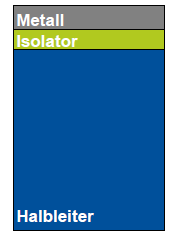
\includegraphics[width=0.2\linewidth]{Kapitel/Kap06/MOSKondensator}
	\end{center}
	
	\subsubsection{Flachbandfall}
		Background: im thermischen Gleichgewicht kommt es zu einem Ausgleich der unterschiedlichen Fermi-Niveaus (Halbleiter und Metall)
		\begin{itemize}
			\item Spannungsunterschied wird als Kontaktpotenzial bezeichnet
			\item 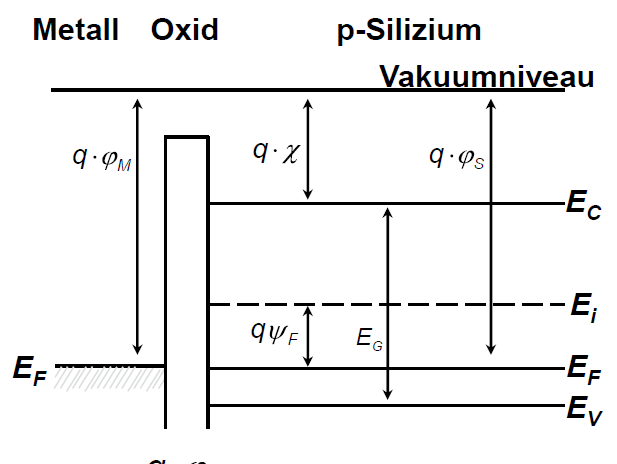
\includegraphics[width=0.4\linewidth]{Kapitel/Kap06/Kontaktpotential} 			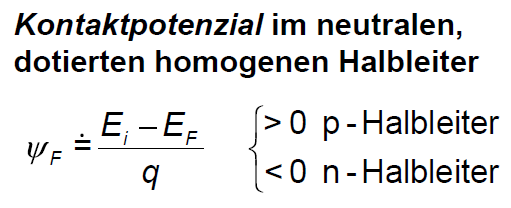
\includegraphics[width=0.4\linewidth]{Kapitel/Kap06/Kontaktpotential2}
			
			\item es bilden sich an der Grenzschicht zwischen Metall und Isolator positive und dem entgegengesetzt an der Grenzschicht zwischen Isolator und Halbleiter negative Ladungen aus.
			\item Es bildet sich eine Raumladungszone im Halbleiter			 		
		\end{itemize}
		Wichtig: Gleicht man das Kontaktpotenzial und den Spannungsabfall über das Oxid durch eine bestimmte schwache 	Vorspannung aus, so verschwindet die Raumladungszone man spricht vom Flachbandfall und der angelegten Flachbandspannung $U_{FB}$.
		
	\newpage
		
	\subsubsection{Anreicherung/Akkumulation, Verarmung, Inversion}
		Arbeitszustände (in diesen Fällen für für p-Silizium Substrate):
		\newline
		!!! Diagramme dienen nur der Veranschaulichung, Inversionsdiagramme sind wichtig !!!!
		\newline
		\textbf{Akkumulation:}
		\newline
		Beim Anlegen einer negative Spannung ($U_{MS} < 0 V $) gegenüber dem Substrat wandern die positiven Ladungsträger im Substrat zur 		Grenzschicht, sammeln sich dort und bilden eine Anreicherungszone
		\newline
		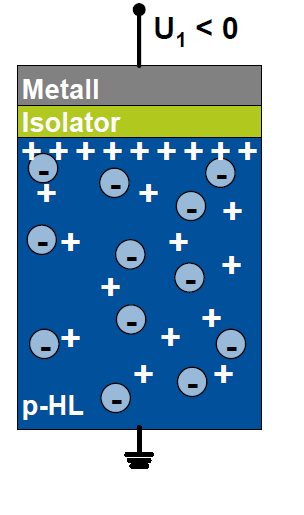
\includegraphics[width=0.25\linewidth]{Kapitel/Kap06/Akkumulation1}		
		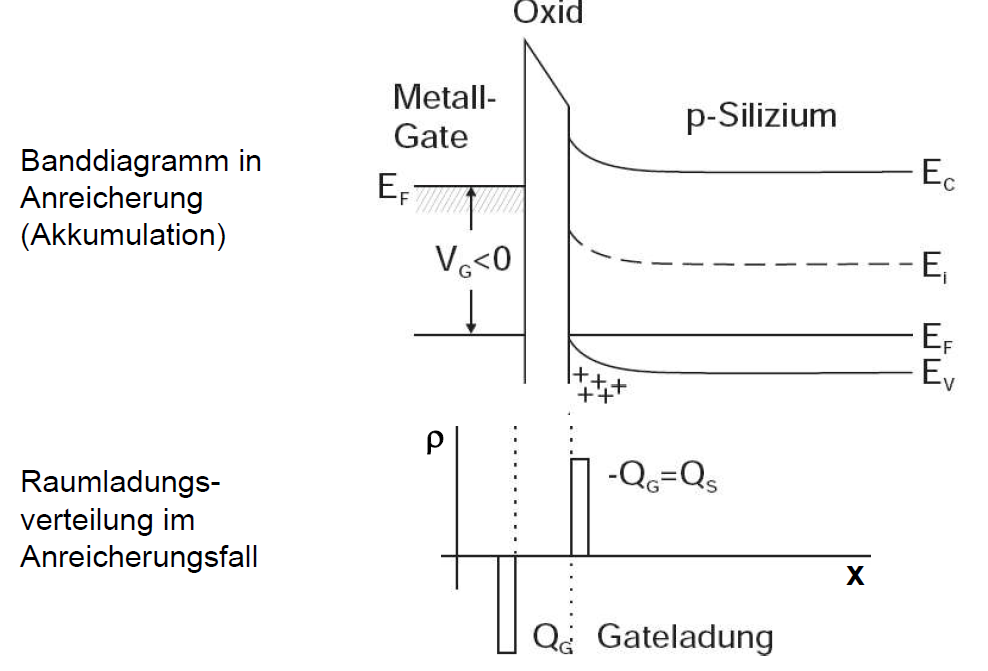
\includegraphics[width=0.60\linewidth]{Kapitel/Kap06/Akkumulation}
		\newline
		\newline
		
		\textbf{Verarmung:}
		\newline
		Bei Anlegen des Pluspols am Metall und
		des negativen Pols am Substrat ($U_{MS} > 0V$) wandern negative Ladungs-träger
		(Minoritäten) im Substrat an die Grenzschicht und rekombinieren mit den dort befindlichen freien positiven Ladungsträgern.
		\newline 
		In der Nähe der Grenzschicht entsteht durch die Rekombinationen eine 		Raumladungszone, die an freien 		Ladungsträgern verarmt ist. Diese Zone wird als Verarmungszone bezeichnet.
		\newline
		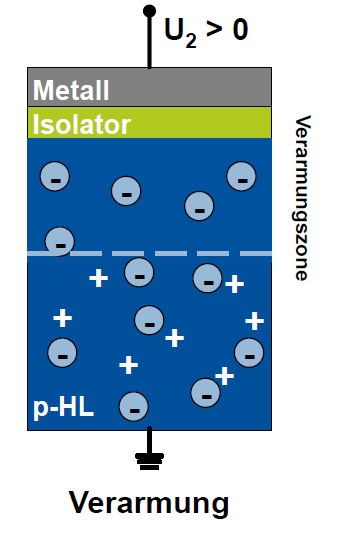
\includegraphics[width=0.25\linewidth]{Kapitel/Kap06/Verarmungszone1}
		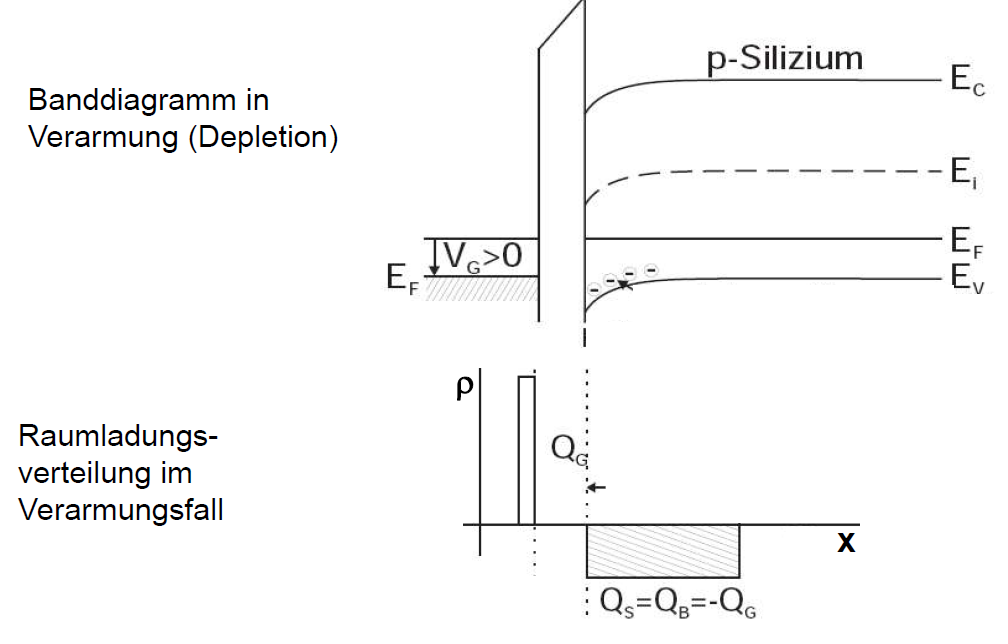
\includegraphics[width=0.60\linewidth]{Kapitel/Kap06/Verarmungszone2}
		
		\textbf{Inverstion:}
		\newline
		Überschreitet die angelegte Spannung eine Schwellspannung ($U_{MS} > U_{th}$ ,Threshold) bildet sich im ursprünglich p-dotierten Substrat ein n-dotiertes Gebiet. Es stehen keine freien Löcher mehr an der Grenzschicht zur Rekombination zur Verfügung.
		\newline
		Die so entstandene Zone, die die frei beweglichen negativen Ladungsträger enthält, wird als Inversionszone 	bezeichnet.
		\newline
		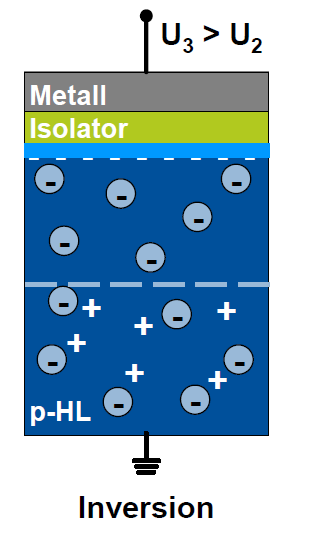
\includegraphics[width=0.25\linewidth]{Kapitel/Kap06/Inverstion1}		
		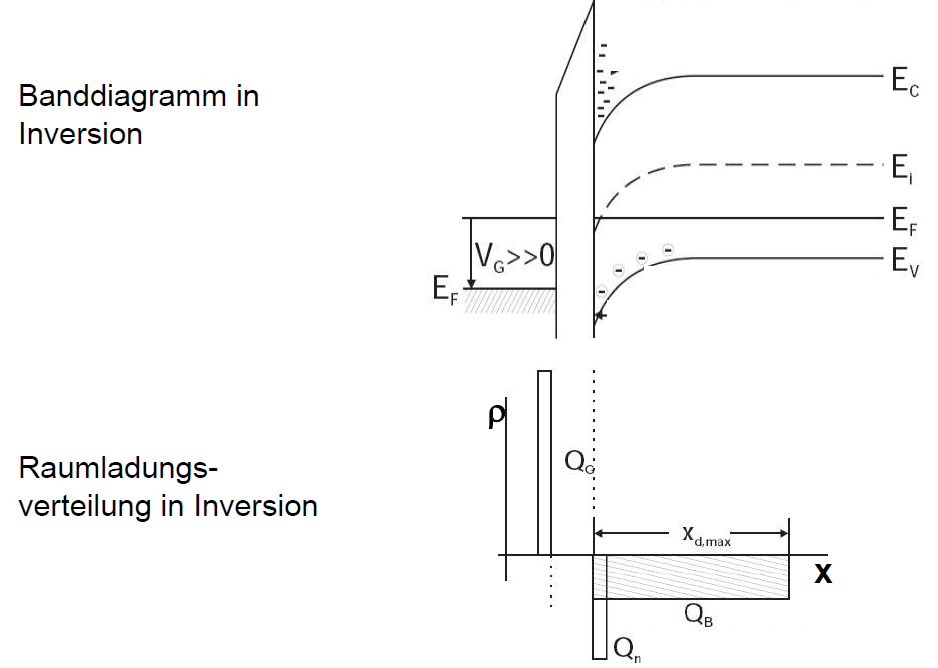
\includegraphics[width=0.60\linewidth]{Kapitel/Kap06/Inversion2}
		
		
\subsection{MOS-Transitoren}
MOS Transistoren sind Feldeffekttransistoren =
MOSFET
	\subsubsection{Grundaufbau}	
	Ein MOSFET ist ein aktives Bauelement mit mindestens drei Anschlüssen:
	\begin{itemize}
		\item S (source, dt. Quelle)
		\item D (drain, dt. Abfluss)
		\item G (gate, dt. Steuerelektrode)
		\item (B (bulk, dt. Substrat), Bei einigen Bauformen wird ein zusätzlicher Anschluss B nach außen geführt. Meistens ist das 		Substrat jedoch intern mit S verbunden )
	\end{itemize}
	Betrieb: Majoritätsladungsträger fließen von S nach D:
	\begin{itemize}
		\item unipolares Bauelement
		\item laterales Bauelement
	\end{itemize}
	Basierend auf dem Feldeffekt wird der Stromfluss wird durch ein an G anliegendes	elektrisches Feld gesteuert.
	\newline
	Die Geschwindigkeit ist vom Ladungsträgertransport von Source zum Drain abhängig. Dabei liegen die heutigen Kanallängen bei < 32 nm.
		%MOS Transistor
		\begin{center}
			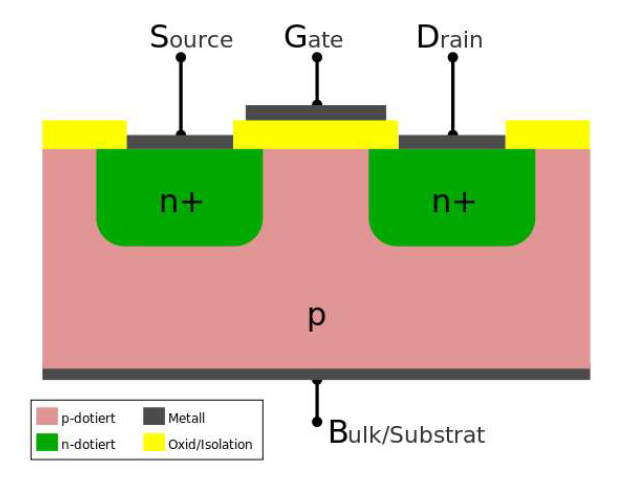
\includegraphics[width=0.7\linewidth]{Kapitel/Kap06/MOS_Transistor.png}
		\end{center}
	\subsubsection{neuere Entwicklungen}
		\textbf{Problem: }
		\newline
		Bei der Skalierung zu neuen Technologiegenerationen wird auch die Gateoxiddicke ebenfalls reduziert. 
		Die Tunnel/Leak-Ströme steigen exponentiell mit abnehmender Dicke.
		Irgendwann wäre man bei 3 Lagen von SiO2-Tetraedern. Die ist technisch nicht mehr homogen realisierbar (min. Schwankung 33 \%), da auch nicht mehr messbar. 
		\newline
		\textbf{Lösung: }
		\newline
		Daher muss trotz Skalierung das Dielektrikum dicker sein. Um die Kapazität bei größerer Dicke beizubehalten werden sogenannte High-K Dielektrika eingesetzt. 
		
		$C = \frac{\epsilon_r  \epsilon_0 A}{d}$ => Wird die Dicke d erhöht muss ein Material mit höherer Dielektrizitätskonstante $\epsilon_r$ (oder amerikanisch K) gefunden werden, um dieses auszugleichen.
	\subsubsection{Die vier Grundtypen}
	\subsubsection{Funktionsweise eines n-Kanal-Anreicherung-Transistoren}
	\subsubsection{Ausgangs- und Transferkennlinien}
\subsection{Anwendungen von MOS-Transistoren}
	
	\subsubsection{Vor- und Nachteile}
	\subsubsection{Funktionsprinzip eines CMOS-Inverter}


\todo{Fragen aus Own Clowd zuordnen}
\todo{Gruppenübungs-Inhalte ergänzen}